\chapter{Rezultati}
\section{Delitev podatkov}
Za končno raziskavo smo imeli na voljo 7368 primerov stanj iz podatkovne zbirke EEG Motor Movement/Imagery Dataset. Primere stanj smo skrčili na enakomerno razporeditev, z 2456 primeri vsakega stanja. Sami smo posneli neka minut posnetkov, 186 primerov stanj od tega 62 primerov vsakega stanja. Za učenje nevronskih mrež smo uporabljali množice za učenje z 75\% podatkov in množice za testiranje z 25\% podatkov.

\section{Izbira metode povezljivosti}
Ker je kompleksni Pearsonov korelacijski koeficient izračunan iz analitičnih signalov ga lahko definiramo samo za ozke frekvenčne pasove. Pri računanju Grangerjevega indexa vzročnosti te omejitve ni, tako da smo ga lahko računali na celotnem frekvenčnem območju do 45Hz. Prav tako se je pojavilo vprašanje koliko dolgo epoho EEG signala bomo potrebovali za uspešno klasifikacijo. Kot možnosti smo vzeli prvo sekundo, prvi dve sekundi, drugi dve sekundi in prve štiri sekunde po dogodku. Točnost klasifikacije smo ocenili z zgoraj navedeno nevronsko mrežo. Za najboljšo metodo se je izkazal kompleksni Pearsonov korelacijski koeficient na območju 13-30Hz z najdalšimi epohami, 4s.
\begin{figure}[h!]
    \begin{center}
    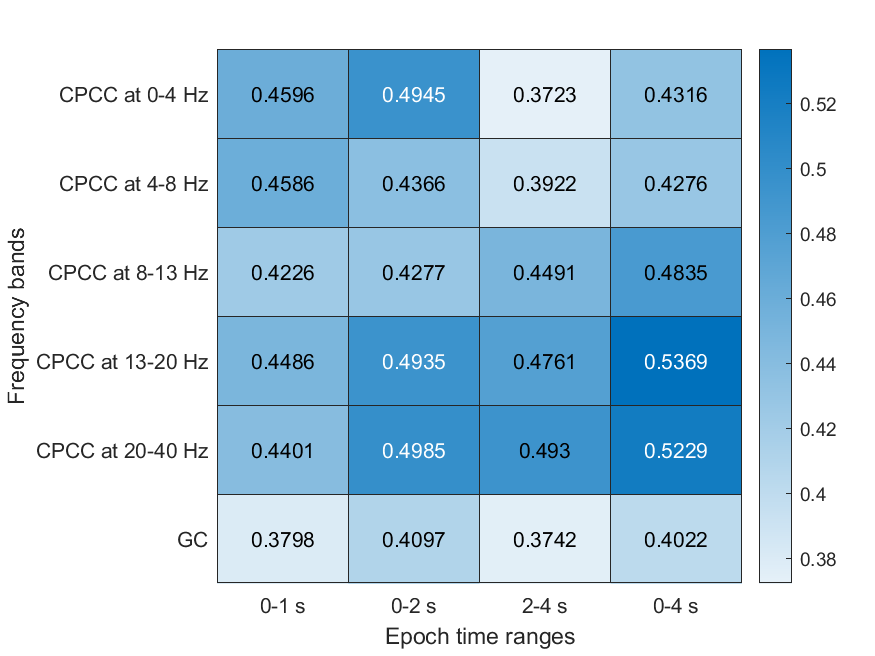
\includegraphics[width=0.5\linewidth]{slike/Comparison.png}
    \end{center}
    \caption{Primerjava območij in dolžin epoh.}
\end{figure}

\section{Primerjava filtrov}
Knjižnica EEGLAB vsebuje samo filtre z ničelno fazo, ki filtrirajo naprej in nato nazaj po času, kar v našem primeru ni primerno saj podatke prejemamo sekvenčno, zato smo podatke filtrirali s pomočjo Butterworthovega filtra ki vsebuje stanja. Stanja nam omogočajo filtriranje sekvenčnih podatkov saj preprečijo napako na začetku filtra kjer le ta potrebuje predpostaviti začetno staje vseh signalov 0. Ker filtra nista enakovredna saj prvi ne spreminja faz drugi pa jih zamakne, uporabljena metoda CPCC pa deluje na zamikih faz, smo izvedli dodatno testiranje, da smo preverili če pristop deluje enako učinkovito.
\begin{figure}[h!]
    \begin{center}
    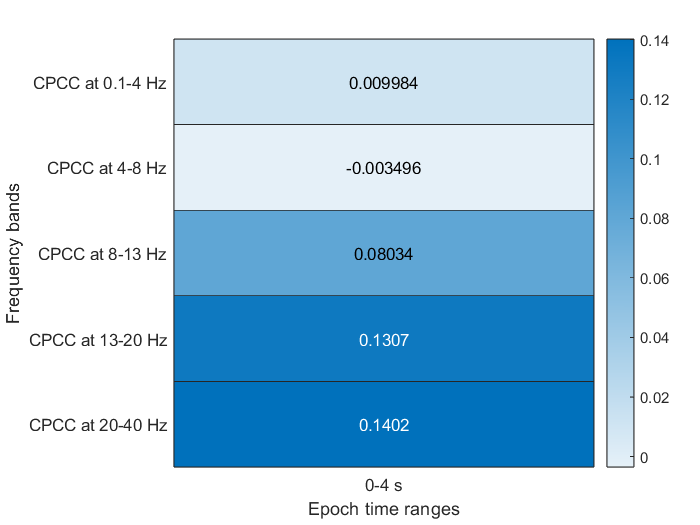
\includegraphics[width=0.5\linewidth]{slike/ComparisonFilters.png}
    \end{center}
    \caption{Primerjava klasifikacije CPCC z nevronsko mrežo za epoho 0-4s za različne frekvenčne pasove \textcolor{red}{ val $= eeglab - Butterworth$ testirano za 30 ljudi * 3 serije} }
\end{figure}

\begin{figure}[h!]
    \begin{center}
    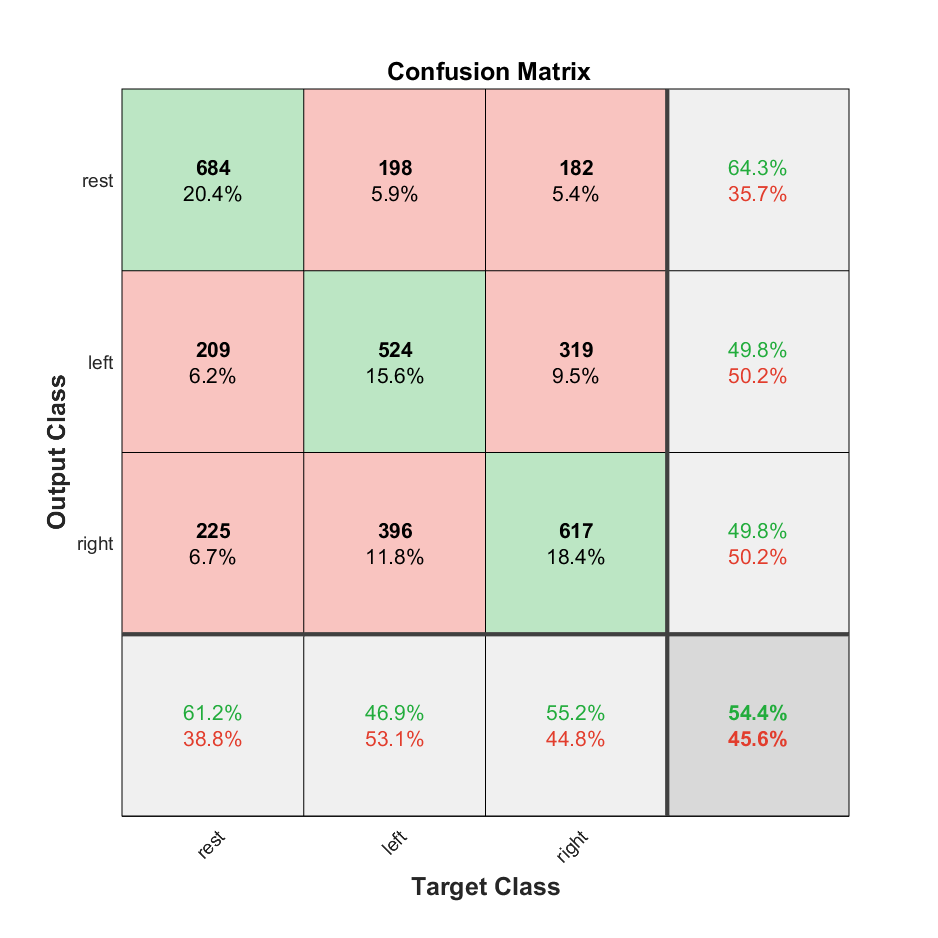
\includegraphics[width=0.5\linewidth]{slike/Confusion_eeglab.png}
    \end{center}
    \caption{Matrika zmede nevronske mreže naučene na podatkih fitriranih s filtrom z ničelno fazo.}
    \end{figure}
    
    \begin{figure}[h!]
    \begin{center}
    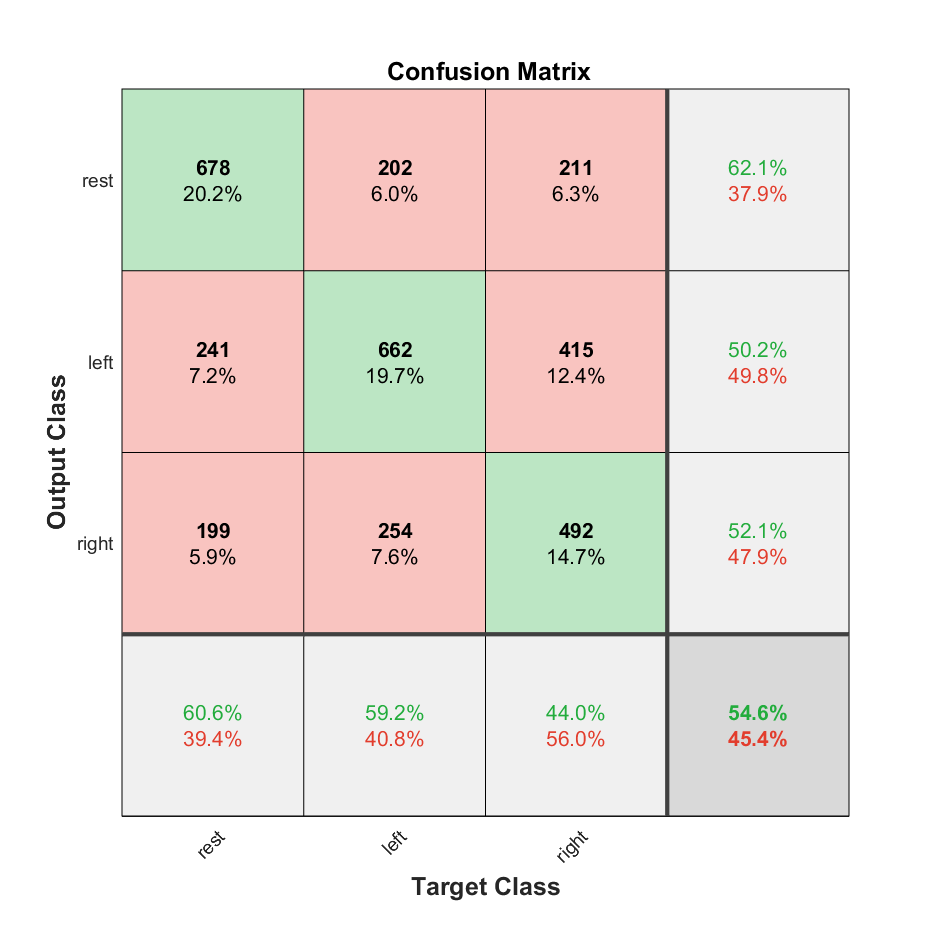
\includegraphics[width=0.5\linewidth]{slike/Confusion_my.png}
    \end{center}
    \caption{Matrika zmede nevronske mreže naučene na podatkih fitriranih z Butterworthovim filtrom.}
    \end{figure}



\section{Rezultati na MMID}
\subsection{Classification learner}
Z uporabo aplikacije clasifiacation learner smo testirali več načinov klasifikacije in dosegl 49\% točnost. 
\begin{table}[h]
\centering
\begin{tabular}{|c|c|}
\hline
Metoda klasifikacije & točnost \\
\hline
odločitvena drevo & 40\%  \\
\hline
k-NN & 41\% \\
\hline
logistična regresija & 49\% \\
\hline
SVM & 45\% \\
\hline
\end{tabular}
\caption{Točnost klasifikacij}
\end{table}

\subsection{Nevronska mreža}
Nato smo poskusili z nevronsko mrežo ki je dosegla 52\% točnost.

\begin{figure}[h!]
\begin{center}
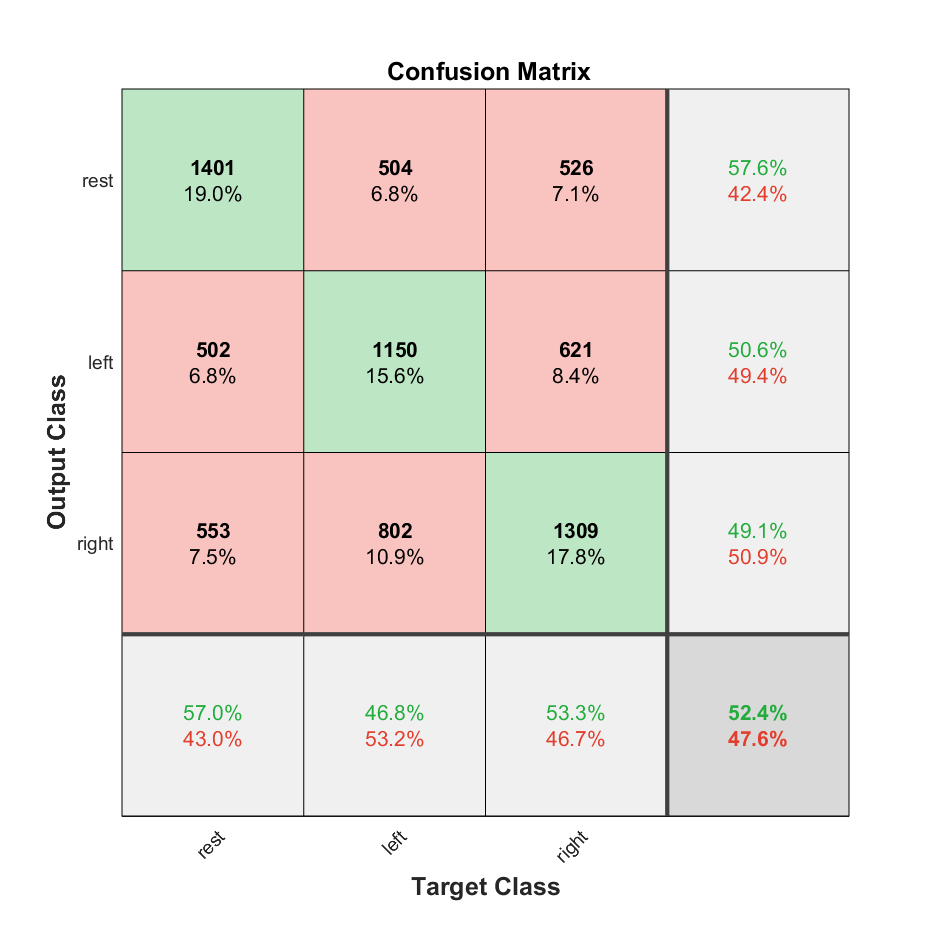
\includegraphics[width=0.5\linewidth]{slike/Confusion_13-20Hz_0s-4s.png}
\end{center}
\caption{Matrika zmede nevronske mreže naučene na podatkih zbirke.}
\end{figure}



\section{Rezultati na lastnih podatkih}
Da bi se približali pogojem v realnem času, smo nevronsko mrežo dodatno naučili na naših podatkih. Zaradi različnih pogojev snemanja in đnčnosti naprav na katerih so podatki snemani je točnost klasifikacije pričakovano padla.
\begin{figure}[h!]
\begin{center}
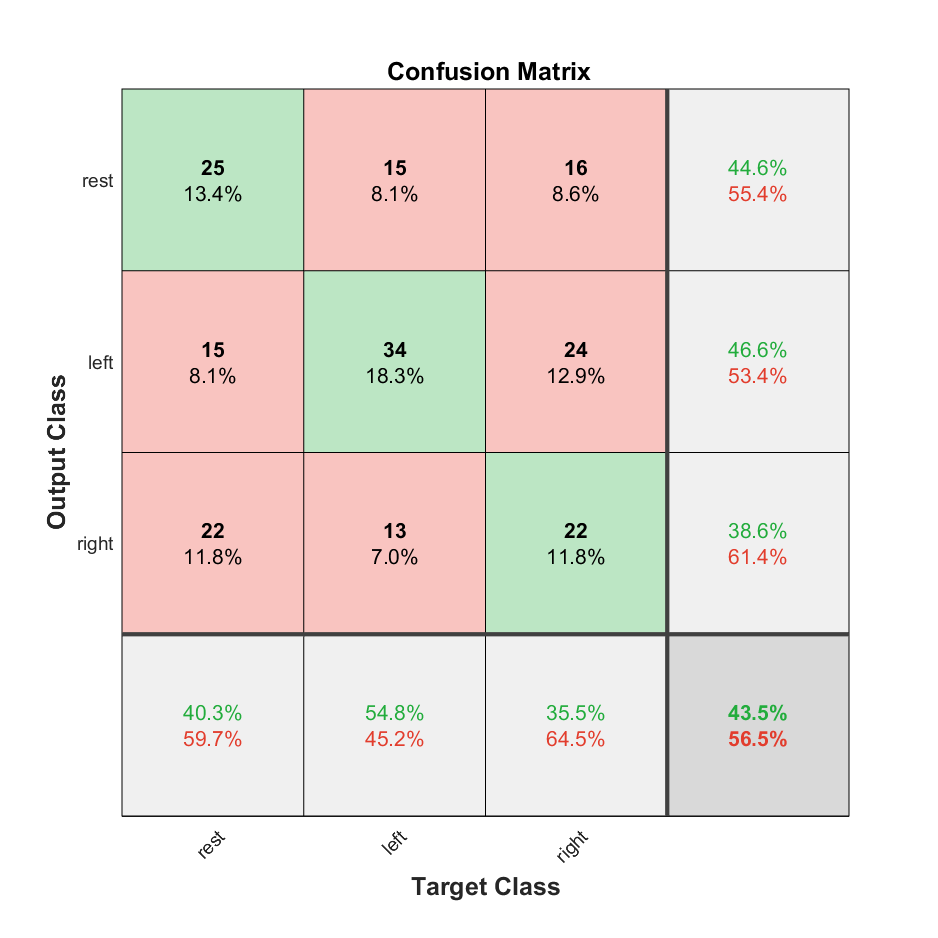
\includegraphics[width=0.5\linewidth]{slike/Confusion_13-20Hz_0s-4s_retrained.png}
\end{center}
\caption{Matrika zmede nevronske mreže dodatno naučene na naših podatkih.}
\end{figure}
\section{Preizkus v realnem času}




